\documentclass[12pt,a4paper]{article}
\usepackage[margin=1in]{geometry} % 设置页面边距
\usepackage{ctex}
\usepackage{graphicx}
\usepackage{float}
\usepackage{amsmath}
\usepackage{amssymb} % 数学符号
\usepackage{booktabs} % 绘制漂亮的表格
\usepackage{array} % 数组和表格
\usepackage{multirow} % 多行合并的表格
\usepackage{caption} % 设置图片和表格的标题格式
\usepackage{subcaption} % 多个子图或表格
\usepackage{parskip}
\setlength{\parindent}{0pt}

\title{\textbf{人工智能导论第一次作业}}
\author{张立博\ 2021012487}
\date{2023.4.1}

\begin{document}

\maketitle

\section{第一题}
\subsection{}
若搜索树的深度为n,每个节点的子节点个数为d\\
DFS:时间复杂度为$O(d^n)$,空间复杂度为$O(dn)$\\
BFS:时间复杂度为$O(d^n)$,空间复杂度为$O(d^n)$\\
\subsection{}
旨在解决树搜索中重复状态和路径冗余的问题,实现上需要多维护一个探索集
\subsection{}
假设约束图有n个变量,每个变量有d个取值,一共有c条边\\
则AC-3算法的最坏时间复杂度为$O(cd^3)$\\
在AC-3算法中,首先将所有约束条件表示为一组弧,然后对每个弧进行处理,直到所有弧都满足弧一致性为止\\
在处理一个弧时,需要检查该弧关联的两个变量的可能取值组合,因此需要进行$O(d^2)$次操作\\
当一个变量失去一个值时需要对周围的弧重新进行检查,由于一个变量有d个值,所以一个弧至少要检查d次\\
一共有c条边,所以最坏时间复杂度为$O(c·d·d^2) = O(cd^3)$
\subsection{}
模拟退火在搜索过程中接受差解,并在一定的概率下接受更劣的解,从而有可能跳出局部最优解并找到全局最优解\\
具体而言,在每个温度下,它从当前解开始,随机选择一个邻居解,并计算其与当前解的差值。如果邻居解更优,则接受该解作为当前解;
如果邻居解更劣,则以一定的概率接受该解。
随着温度的逐渐降低,接受更劣解的概率逐渐减小,最终搜索收敛于全局最优解。
\section{第二题}
\begin{figure}[H]
    \centering
    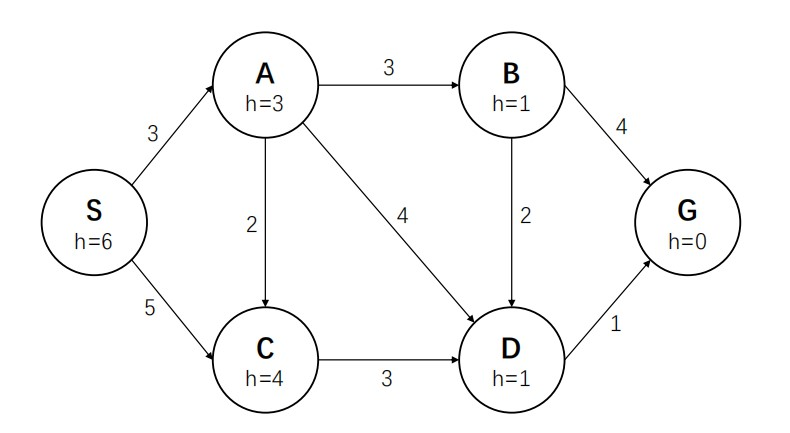
\includegraphics[scale = 0.8]{2.jpg}
    \label{figure}
\end{figure}
\subsection{UCS}
\begin{figure}[H]
    \centering
    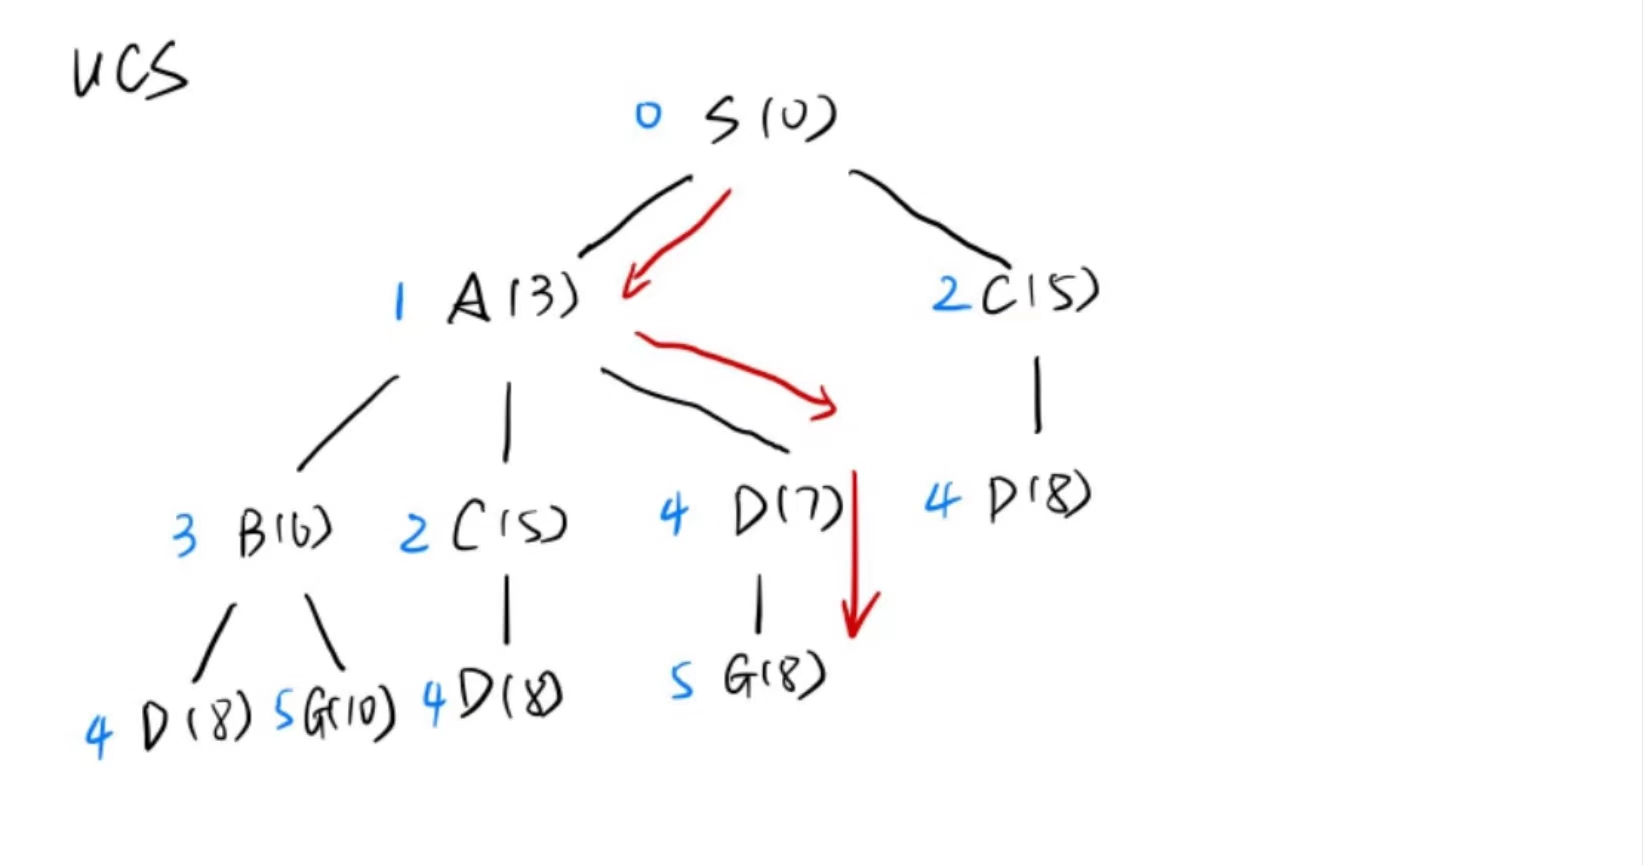
\includegraphics[scale = 0.2]{ucs.jpg}
    \label{figure}
\end{figure}
搜索树如上,字母表示节点,右侧数字表示代价值,左侧序号表示被探索的次序,红色为最优路径\\
最优路径为$S\rightarrow A \rightarrow D\rightarrow G$
\subsection{Greedy}
\begin{figure}[H]
    \centering
    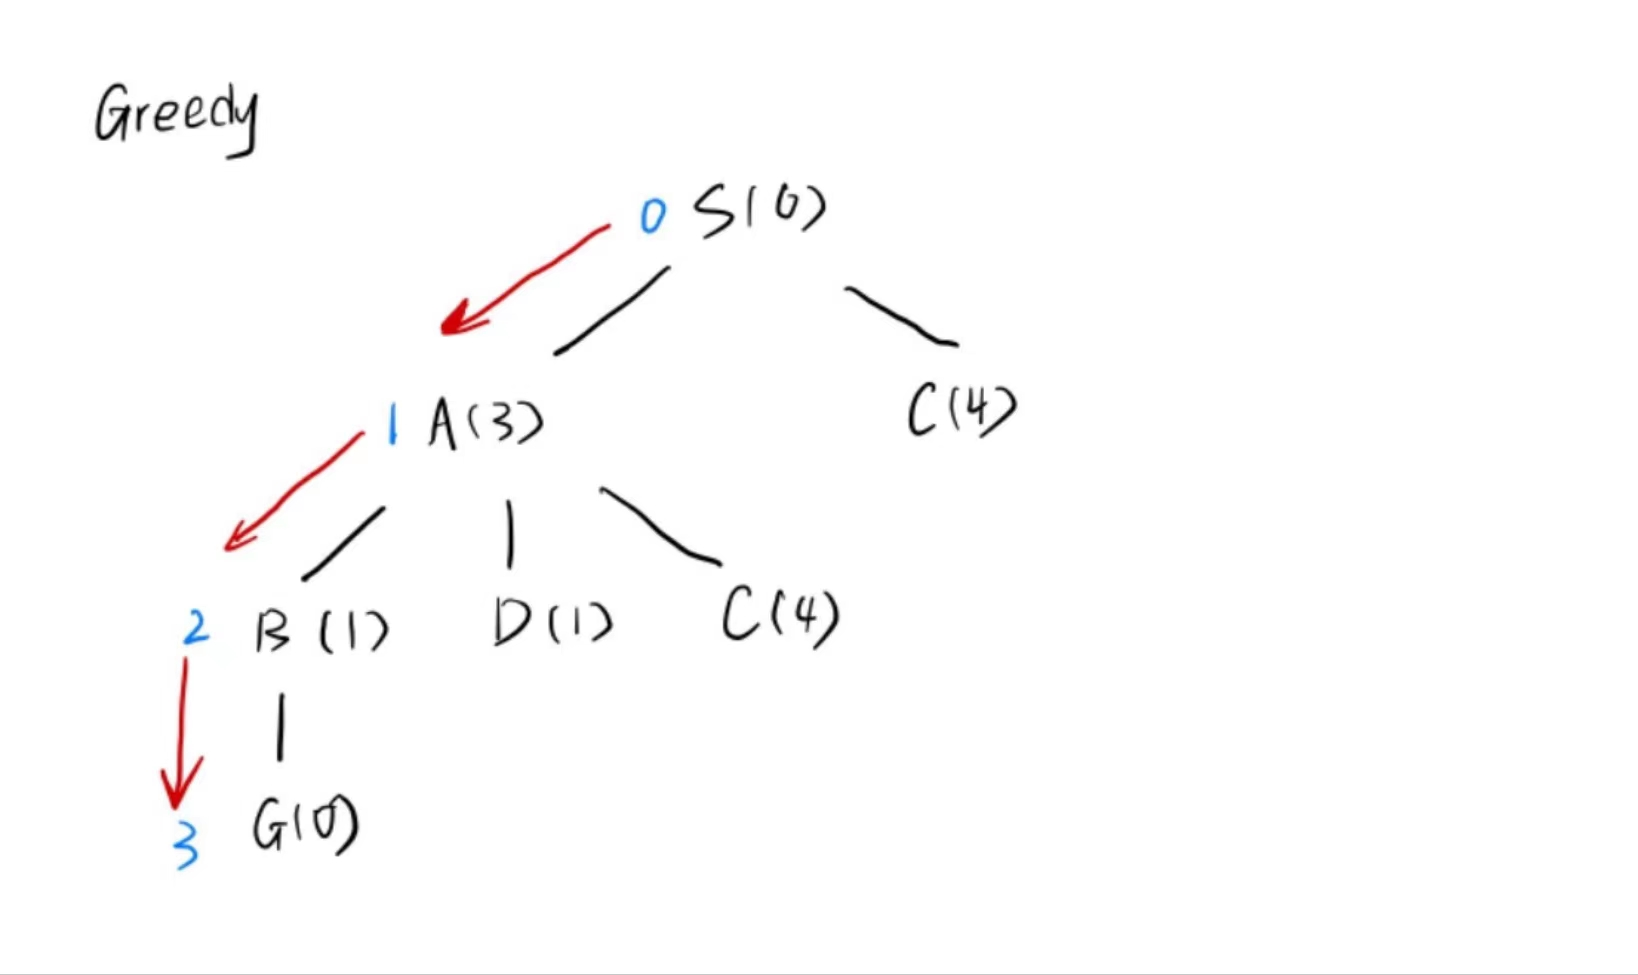
\includegraphics[scale = 0.2]{greedy.jpg}
    \label{figure}
\end{figure}
搜索树如上,字母表示节点,右侧数字表示启发值,左侧序号表示被探索的次序,红色为最优路径\\
最优路径为$S\rightarrow A \rightarrow B\rightarrow G$
\subsection{A*}
\begin{figure}[H]
    \centering
    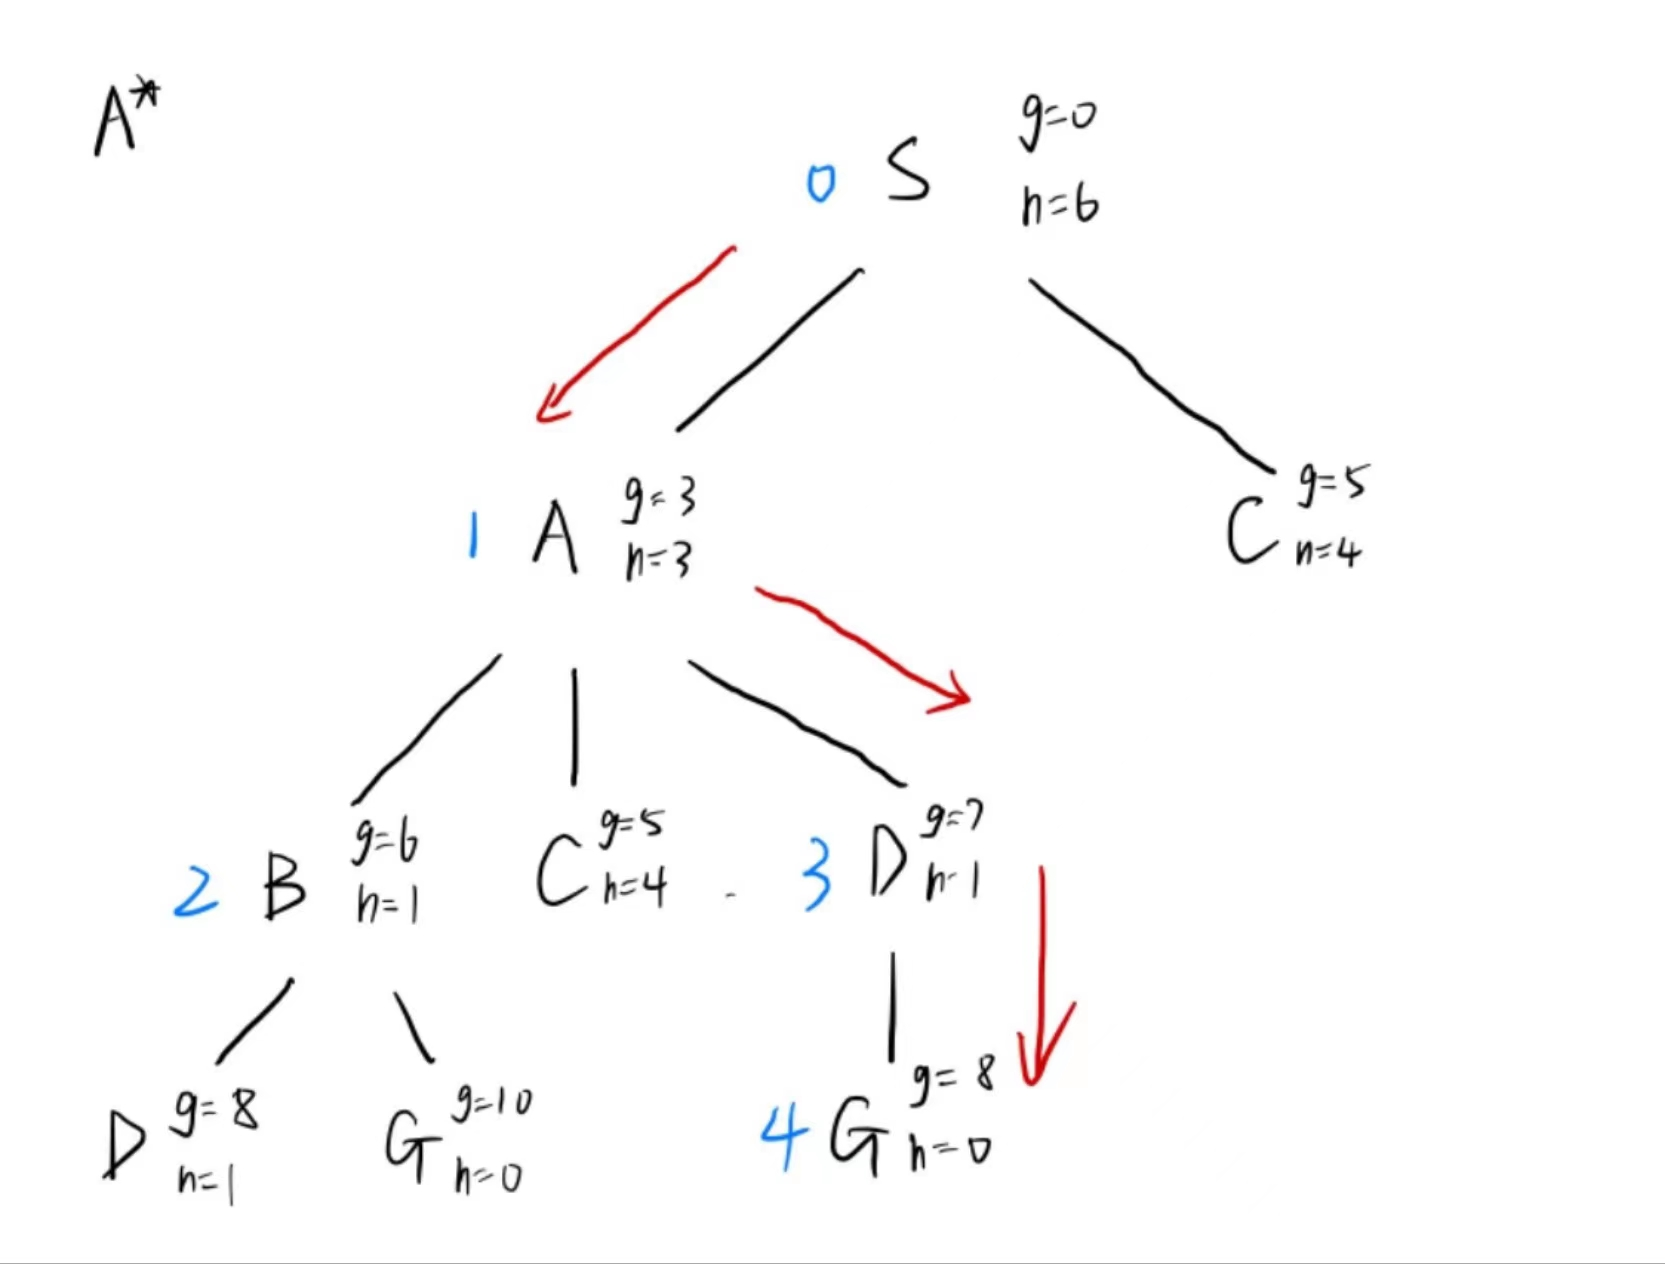
\includegraphics[scale = 0.2]{A.jpg}
    \label{figure}
\end{figure}
搜索树如上,字母表示节点,右侧数字表示代价值和启发值,左侧序号表示被探索的次序,红色为最优路径\\
最优路径为$S\rightarrow A \rightarrow D\rightarrow G$
\section{第三题}
设在一个搜索过程中,n是m的子节点\\
则由$f(n)$递增得
\begin{align*}
    f(m) \leq f(n)
\end{align*}
\begin{align*}
    g(m) + W\cdot h(m) \leq g(n) + W\cdot h(n)\\
\end{align*}
设$c(m,n)$为m到n的代价值,则
\begin{align*}
    g(m) + W\cdot h(m) \leq g(m) + c(m,n) + W\cdot h(n)\\
\end{align*}
即
\begin{align*}
    h(m) - h(n) \leq \frac{c(m,n)}{W}
\end{align*}
因$W>1,c(m,n)\geq 0$\\
所以
\begin{align*}
    h(m) - h(n) \leq \frac{c(m,n)}{W} \leq c(m,n)
\end{align*}
又$h(T) = 0$,所以$h(n)$单调,则A*扩展了节点n之后,就找到了到达节点n的最佳路径\\
所以
\begin{align*}
    g^*(n) = g(n)
\end{align*}
$g^*(n)$为从节点S到节点n的最短路径的代价值\\
设节点x为从S到T的最短路径上T的祖先(也可能是T自己)\\
则
\begin{align*}
    h^*(S) = g^*(x) + h^*(x) = g(x) + h^*(x)
\end{align*}
又$h(x)\leq h^*(x)$\\
所以
\begin{align*}
    h^*(S) \geq g(x) + h(x)
\end{align*}
又$W > 1,g(x) \geq 0$\\
所以
\begin{align*}
    W\cdot h^*(S) \geq W\cdot g(x) + W\cdot h(x) \geq g(x) + W\cdot h(x) = f(x)
\end{align*}
令$x = T$
则
\begin{align*}
    W\cdot h^*(S) \geq f(T) = g(T) + W\cdot h(T) = g(T)
\end{align*}
综上
\begin{align*}
    g(T)\leq W\cdot h^*(S)
\end{align*}
\end{document}